\part{Les nombres premiers}
\setcounter{section}{0}
\section{Définition et histoire}
\begin{definition}
\label{def:nb_prem}
Un entier n supérieur ou égal à deux est dit premier si et seulement si ses seuls diviseurs positifs sont 1 et lui-même.
\end{definition}

\begin{theorem} \label{thm:InfPre}
Il y a une infinité de nombres premiers.
\end{theorem}


\begin{proof}
Nous allons maintenant démontrer par l'absurde qu'il existe une infinité de nombres premiers. \\
Supposons que P soit fini, de cardinal n. Soient $p_1,...,p_n$ ses éléments. \\
Posons $N= 1 + p_1 ... p_n$. On a $N \geq 2$, donc N possède un diviseur premier p (d'apres \ref{itm:divprem}). \\
L'entier p divise $p_1 ... p_n$, d'où l'on déduit que p divise 1. Cela conduit à une contradiction. P est donc infini.
\end{proof}

\begin{history} \ref{histoire}
On peut retrouver des traces des nombres premier à 20 000 ans avant notre ère, sur l'os d'Ishango où figurent les nombres 11, 13, 17 et 19. \\
Durant l'antiquité, Euclide met en place des théories et des affirmations dans les "Eléments", ainsi que la décomposition en facteurs premiers. Puis, ce sera Eratosthène de Cyrène qui donnera une méthode simple pour déterminer les nombres premiers. \\
Par la suite, au Moyen-Age, ce sera Fibonnacci qui en fera une liste et en déterminera des critères de divisibilité. Ce sera un ecclésiastique français du nom de Marin Mersenne qui posa la question : si p est premier est-ce que $2^p - 1$ est premier ? Il a été montré que non, cependant la méthode est encore utilisée pour déterminer les nombres premiers dits "géants". \\
Ce sera ensuite durant la Renaissance que Goldbach affirmera que tout nombre peut s'écrire sous forme d'une somme de deux nombres premiers. Euler quant à lui prouvera que $2^{31} - 1$ est premier. Gauss et Legendre vont par la suite s'intéresser à la repartition des nombres premier, montrant que plus les nombres sont dits "géants", moins les nombres premiers seront présents. \\
Aujourd'hui, le plus grand nombre premier connu a été decouvert en 2018 et est : $2^{82 \ 589 \ 933} - 1$.
\end{history}


\section{Le théorème fondamental de l'arithmétique}

Concernant les nombres premiers, les deux théorèmes à la fois les plus importants et les plus anciens, sont : \newline
-Il y a une infinité de nombres premiers (Théorème \ref{thm:InfPre}). \newline
-Le théorème fondamental de l'arithmétique.

\begin{theorem}
\textbf{Théorème fondamental de l'arithmétique} : \newline
Tout entier $n > 0$ peut être écrit comme un produit de nombres premiers, de façon unique.
\end{theorem}

De ce théorème s'ensuivent un corollaire et une définition :

\begin{corollary}
\textbf{Nombres premiers} : \newline
Un nombre est premier si et seulement si il est l'unique facteur de sa décomposition.
\end{corollary}

\begin{definition}
\textbf{Nombres composés} : \newline
Un entier $n > 0$ est dit composé si et seulement si il est le produit d'au moins $2$ nombres.
\end{definition}

Regardons quelques exemples pour bien comprendre comment marche une décomposition : 

\begin{example}
: \newline
- $6 \ 936 = 2^{3} \times 3 \times 17^{2}$ \newline
- $1 \ 200 = 2^{4} \times 3 \times 5^{2}$ \newline
- $7 = 7$ \newline
Les deux premiers nombres sont donc des nombres composés tandis que le dernier nombre est premier.
\end{example}

(La manière dont on trouve ces décompositions sera vue plus en profondeur dans les sections \ref{sec:algo_euclide} et \ref{sec:Algorithme})


\subsection{démonstration}

Pour démontrer le Théorème fondamental de l'arithmétique, il est nécessaire de le diviser en 2 parties. \newline
En effet, le théorème affirme l'existence d'une décomposition ; et l'unicité de cette dernière. \newline
Il nous faudra donc prouver son existence, et ensuite prouver que cette décomposition est unique. \newline
(La démonstration est issue d'une vidéo youtube \ref{itm:FunAri})

\subsubsection{Partie 1 : existence de la décomposition}

\begin{proof}
Nous ferons une démonstration par l'absurde : \newline
Supposons qu'il existe au moins un entier naturel qui ne possède \textbf{pas} une telle décomposition.\newline
On pose $m$, le plus petit de ces entiers. \newline
On observe que $m$ est forcément composé (sinon il serait premier et, par définition, serait sa propre décomposition). \newline
\newline
On pose donc, \newline
$$ m = ab \ \ \ \ \text{avec} \ 1 < a,b < m$$ 
Vu que $a,b < m$, on peut écrire $a$ et $b$ dans leur décomposition (car on a posé m comme étant \textbf{le plus petit} entier qui ne peut pas s'écrire sous cette forme). \newline
Donc :

\begin{equation*} \label{equ:a}
    a = p_1^{\alpha_1} \ldots p_n^{\alpha_n} \ \ \ \ p_i \ premiers \ / \ \alpha_i \in \ens{N} \ \ (1 \leq i \leq n)
\end{equation*}
\begin{equation*} \label{equ:b}
    b = q_1^{\beta_1} \ldots q_m^{\beta_m} \ \ \ \ q_i \ premiers \ / \ \beta_i \in \ens{N} \ \ (1 \leq i \leq m)
\end{equation*}
\newline
mais par définition de $m$, on a :
\begin{align*}
    m & = ab \\
      & = p_1^{\alpha_1} \ldots p_n^{\alpha_n} \times q_1^{\beta_1} \ldots q_m^{\beta_m} \\
\end{align*}
$m$ possède donc une décomposition en facteurs premiers, ce qui contredit le prédicat. \newline
Par conséquent, on conclut qu'il n'existe pas d'entier naturel $m$ qui ne possède pas de décomposition en facteurs premiers.
\end{proof}

\subsubsection{Partie 2 : unicité de la décomposition}

Avant de s'attaquer à l'unicité, nous devons d'abord introduire le lemme d'Euclide :

\begin{lemma}
\textbf{Lemme d'Euclide} : \newline
Soient $b,c \in \ens{N}$. \newline
Si un nombre premier $p$ divise le produit $b \times c$, alors $p$ divise $b$ \textbf{ou} $p$ divise $c$.
\end{lemma}

\begin{proof}
Voir la référence \ref{itm:LemEuc}.
\end{proof}

Maintenant que cela a été posé, commençons la démonstration de l'unicité de la décomposition en facteurs premiers :

\begin{proof}
Nous ferons aussi une démonstration par l'absurde : \newline
Supposons que $2$ décompositions différentes sont égales :
\begin{equation*}
    p_1^{\alpha_1} \ldots p_n^{\alpha_n} = q_1^{\beta_1} \ldots q_m^{\beta_m}
\end{equation*}
Nous avons 3 objectifs : \newline
1) Montrer que $n=m$. \newline
2) Montrer que $p_i=q_i \ \ (\forall i, \ 1 \leq i \leq n,m)$. \newline
3) Montrer que $\alpha_i=\beta_i \ \ (\forall i, \ 1 \leq i \leq n,m)$. \newline
\newline
Premièrement, on sait que :
$$p_i \ \text{divise} \ p_1^{\alpha_1} \ldots p_n^{\alpha_n} \ \ (\forall i, \ 1 \leq i \leq n)$$
mais par conséquent,
$$p_i \ \text{divise aussi} \ q_1^{\beta_1} \ldots q_m^{\beta_m} \ \ (\forall i, \ 1 \leq i \leq n)$$ 
(vu qu'ils sont censés être égaux) \newline

Mais si on applique plusieurs fois le lemme d'Euclide, on déduit que :
\begin{align*}
    & p_i \ \text{divise} \ q_r^{\beta_r} \ (\text{pour un certain} \ 1 \leq r \leq m) \\
    \implies & p_i \ \text{divise} \ q_r \\
\end{align*}
(Note : Si ces deux assertions ne vous paraissent pas évidentes, il faut comprendre que le lemme d'Euclide s'étend à autant de facteurs que vous le voulez. Vu que $p_i$ divise la décomposition de facteurs premiers, alors on sait que $p_i$ divise \textbf{au moins un} des facteurs, d'où la précision de "un \textbf{certain} $r$". \newline
Et vu que $p_i$ divise un nombre mis à une puissance, ce nombre n'a comme facteurs que lui même, d'où l'implication que $p_i$ divise $q_r$) \newline
\newline
Maintenant on sait que que $p_i$ divise $q_r$, mais on rappelle que $p$ et $q$ sont des nombres \textbf{premiers}.\newline
Par conséquent, ils ne possèdent aucun diviseur autre que 1 et eux-même, et vu que $p,q \not= 1$ (car $1$ n'est pas considéré comme premier), on conclut que :
$$p_i=q_r$$
Mais si l'on répète ce processus pour chaque facteur des deux côtés de l'égalité, alors on observe qu'à chaque facteur $p_i$ on peut associer un facteur $q_r$, et inversement. \newline
Par conséquent, on conclut que :
$$n=m$$
et que les deux décompositions possèdent les mêmes nombres premiers en facteurs. \newline
\newline
Maintenant que nous avons prouvé que les deux décompositions ont le même nombre de facteurs, et que ces facteurs sont égaux entre eux, il suffit de prouver que ces facteurs sont bien élevés aux mêmes puissances. \newline
Après avoir réarrangé les termes, on a :
\begin{equation} \label{equ:Facteurs}
    p_1^{\alpha_1} \ldots p_n^{\alpha_n} = p_1^{\beta_1} \ldots p_n^{\beta_n}
\end{equation}
On cherche donc à montrer que :
$$\alpha_i = \beta_i \ \ (\forall i, \ 1 \leq i \leq n)$$
\newline
Nous allons démontrer cela par l'absurde : \newline
Assumons que $\alpha_i > \beta_i$ \newline
Divisons les deux côtés de l'égalité (\ref{equ:Facteurs}) par $p_i^{\beta_i}$. On obtient donc l'égalité suivante :
\begin{equation} \label{equ:Division}
    p_1^{\alpha_1} \ldots p_i^{\alpha_i-\beta_i} \ldots p_n^{\alpha_n} = p_1^{\beta_1} \ldots p_{i-1}^{\beta_{i-1}} p_{i+1}^{\beta_{i+1}} p_n^{\beta_n}
\end{equation}
(Note : si vous n'avez pas bien compris, vu que $\alpha_i > \beta_i$, alors du côté gauche le facteur $p_i$ existe toujours, il a juste perdu en puissance, alors qu'à droite il a tout simplement disparu, emporté par la division.) \newline
\newline
Avec l'égalité (\ref{equ:Division}), on en déduit :
\begin{align*}
    & p_i \ \text{divise} \ p_1^{\alpha_1} \ldots p_i^{\alpha_i-\beta_i} \ldots p_n^{\alpha_n} \\
    \implies & p_i \ \text{divise} \ p_1^{\beta_1} \ldots p_{i-1}^{\beta_{i-1}} p_{i+1}^{\beta_{i+1}} p_n^{\beta_n} \\
    \implies & p_i \ \text{divise} \ p_j \ \ \ \text{avec} \ i \not= j 
    \ \ \ \text{\scriptsize{(D'après le lemme d'Euclide)}} \\
\end{align*}
Mais nous sommes face à une contradiction ! \newline
En effet, $p_i$ \textbf{ne peut pas} diviser $p_j$, car ces deux nombres ont été définis comme premiers. \newline
On en conclut donc que, $$\alpha_i \not> \beta_i$$ et avec la logique inverse on pourrait aussi prouver que, $$\alpha_i \not< \beta_i$$
\newline
Conclusion : $$\alpha_i = \beta_i \ \ (\forall i, \ 1 \leq i \leq n)$$
\newline
\newline
Nous avons démontré que si deux décompositions sont égales, alors cela implique qu'elles aient le même nombre de facteurs, que ces facteurs soient égaux entre eux, et que ces mêmes facteurs soient élevés à une même puissance. De cela nous pouvons enfin conclure que :
\begin{center}
    \textbf{La décomposition d'un nombre en facteurs premiers est unique.}
\end{center}

\end{proof}


\subsection{Forme générale d'une décomposition}
\label{sec:Decompo}

Maintenant que nous avons fini la démonstration, nous pouvons enfin énoncer le théorème :

\begin{theorem}
\textbf{Théorème fondamental de l'arithmétique} : \newline
$\forall n \in \ens{N} \backslash \{0,1\}$, $\exists! k \in \ens{N}^{*}$ avec $p_1 \ldots p_k$ des nombres premiers et \newline $\alpha_1, \ldots ,\alpha_k \in \ens{N}^{*}$ tel que :
$$n = p_1^{\alpha_1} \ldots p_k^{\alpha_k}$$
\end{theorem}

(Nous verrons des applications de ce théorème dans les sections \ref{part:pgcd_decompo} et \ref{part:ppcm_decompo})


\section{Deux outils de l'arithmétique}
\subsection{Le PGCD : Plus Grand Commun Diviseur}
\begin{definition} \normalfont
Soient a et b deux entiers dont au moins l'un des deux est non nul. On appelle \red{PGCD} le \red{P}lus \red{G}rand \red{C}ommun \red{D}iviseur de a et b. On note $a \bigwedge b$ le plus grand des diviseurs communs à a et b.
\end{definition}

\begin{property} \normalfont
Montrons quelques propriétés du PGCD : 
\begin{enumerate} \normalfont
\item $\forall a \in \mathbb{N}^*$, PGCD(a,0) = a et PGCD(a,1) = 1
\item PGCD(a,b) = PGCD (b,a)
\item \label{prop:homopgcd}
Si $ (a,b,k) \in \mathbb{Z}^3$, $(ka) \bigwedge (kb) = |k|(a \bigwedge b)$, cela représente l'homogénéité du PGCD. Soit PGCD(ka,kb) = k $\times$ PGCD(a,b)
\item Si b $\in \mathbb{N}^*$, et si a = bq + r est la division euclidienne de a par b, alors $a \bigwedge b = b \bigwedge r$
\item Pour tout couple $(a,b) \in \mathbb{Z}^2$, il existe $(u,v) \in \mathbb{Z}^2$ tel que : \\
$au + bv = a \bigwedge b$. Le couple (u,v) est appelé couple de coefficient de Bezout. \\
Si $au + bv = 1$, on peut déduire que a et b sont premiers entre eux, c'est à dire que a ne divise pas b, et reciproquement que b ne divise pas a.
(On appelle cette propriété : "Théorème de Bachet-Bézout"\ref{itm:ThmBaBe})
\end{enumerate}
\end{property}

\begin{example} \normalfont
Voici quelques exemples de PGCD:
\item PGCD(60,100) = 20
\item PGCD(252,360) = 36 
\item PGCD(2730,5610) = 30
\end{example}


\subsubsection{L'Algorithme d'Euclide} \normalfont
\label{sec:algo_euclide}

\begin{definition} \normalfont
L'Algorithme d'Euclide est un algorithme permettant de calculer facilement le PGCD de deux nombres a et b. Pour cela, il faut calculer la division euclidienne de a par b. Ensuite a prend la valeur de b et b prend la valeur du reste. On répète l'opération jusqu'à ce que b soit égal à 0. On prend alors la valeur (finale) de a. \newline
Pour mieux comprendre ce propos, en voici une illustration (Figure \ref{fig:euclide}) ainsi qu'un exemple.

\begin{example} \normalfont
PGCD(360, 252): \newline
$360 = 252 \times 1 + 108$ \newline
$252 = 108 \times 2 + 36$ \newline
$108 = 36 \times 3 + 0$ \newline
Le PGCD de 360 et 252 est 36.
\end{example}

\begin{figure}[h]
    \centering
    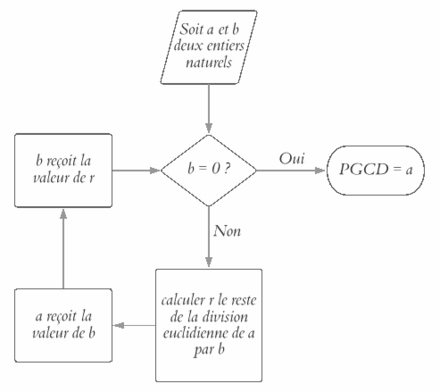
\includegraphics[scale=0.5]{algo.jpg}
    \caption{Algorithme Euclide}
    \label{fig:euclide}
\end{figure}

\end{definition}
\subsection{Le PPCM : Plus Petit Commun Multiple}
Le \red{PPCM} signifie \red{P}lus \red{P}etit \red{C}ommun \red{M}ultiple.

\begin{definition}
Soient a et b deux entiers. Les assertions suivantes sont équivalentes :
\begin{itemize}
    \item a est un multiple de b
    \item b est un diviseur de a
    \item b|a
    \item $\exists k \in \ens{Z} \ \text{tel que} \ bk = a$
\end{itemize}
\end{definition}
Le PPCM de deux entiers a et b, noté $a \vee b$, est donc le plus petit entier naturel qui soit à la fois un multiple de a et de b.

\begin{example}
$3 \vee 5 = 15$ ; $2 \vee 6 = 6$
\end{example}

Bien que moins étudié que le PGCD, le PPCM possède néanmoins lui aussi quelques propriétés intéressantes.

La plus notable est la suivante :

\begin{theorem}
Soient $m = a \vee b$, et q un entier. On a alors :\\
$(a|q)$ et $(b|q) \iff (m|q)$
\end{theorem}

\subsection{Liens avec la décomposition en facteur premier}
\subsubsection{Calculer le PGCD à partir de la décomposition en facteurs premiers}
\label{part:pgcd_decompo}

Avoir la décomposition en facteurs premiers de deux nombres a et b permet de calculer très facilement leur PGCD $a \wedge b$.

Il suffit d'étudier chaque facteur commun aux décompositions de a et b, et de le prendre au plus petit exposant. En multipliant tous les facteurs retenus, nous obtenons le PGCD de a et b.

Prenons un exemple :

\begin{example}

Posons $a = 792 \ et \ b = 2970$. On a :\\
$a = 2^3 \times 3^2 \times 11$\\
$b = 2 \times 3^3 \times 5 \times 11$\\
Il devient très facile de calculer $a \wedge b = 2 \times 3^2 \times 11 = 198$.

\end{example}

Pour effectuer ce calcul, le raisonnement fut le suivant :

\begin{itemize}
    \item 2 est un factuer commun aux décompositions de a et b. Dans la décomposition de a, il est à l'exposant 3, tandis qu'il est exposant 1 dans la décomposition de b. Nous prenons le plus petit exposant, on garde donc $2^1 = 2$.
    \item 3 est également un facteur commun aux deux décomositions. Il est au plus petit exposant dans celle de a, on retient donc $3^2$.
    \item 5 n'est pas présent dans la décomposition de a, on ne le garde donc pas.
    \item 11 est un facteur commun aux deux décomposition. Il est en outre à l'exposant 1 dans les deux cas. On garde donc $11^1 = 11$.
\end{itemize}

D'où, en faisant le produit, $a \wedge b = 2 \times 3^2 \times 11$.\\
\\

\begin{proof}
Le fonctionnement de cette méthode est assez intuitif, quand on comprend le sens de la décomposition en facteurs premiers. Une façon de le démontrer serait d'appeler m le nombre que nous trouvons avec cette technique, et d'ensuite étudier a et b divisés par m.

On remarquerait alors que a/m et b/m n'ont pas de diviseur commun autre que 1.
D'après la propriété \ref{prop:homopgcd} :

$a \wedge b = (m \frac{a}{m}) \wedge (m \frac{b}{m}) = |m|(\frac{a}{m} \wedge \frac{b}{m}) = m \times 1 = m$
\end{proof}

\subsubsection{Calculer le PPCM à partir de la décomposition en facteurs premiers}
\label{part:ppcm_decompo}

La décomposition en facteurs premiers permet aussi, via une méthode à peu près similaire à celle vue ci-dessus, de calculer le PPCM de deux nombres.

La différence avec la méthode de calcul du PGCD est que, pour chaque facteur présent dans la décomposition en facteurs premiers de a \textbf{OU} b, on garde l'exposant le plus \textbf{grand}.

Reprenons l'exemple ci-dessus :

\begin{example}
Prenons encore :\\
$a = 792 = 2^3 \times 3^2 \times 11$ et \\
$b = 2970 = 2 \times 3^3 \times 5 \times 11$\\
On calcule alors :
$a \vee b = 2^3 \times 3^3 \times 5 \times 11 = 11 \ 880$.
\end{example}

\subsection{Lien entre PGCD et PPCM}
Une formule simple relie le PPCM et le PGCD de deux nombres :

\begin{theorem}
\label{thm:rap_pgcd_ppcm}
\begin{align*}
& PGCD(a, b) \times PPCM(a, b) = |ab| \\
& \iff PGCD(a, b) = \frac{|ab|}{PPCM(a, b)} \\
& \iff PPCM(a, b) = \frac{|ab|}{PGCD(a, b)}
\end{align*}
\end{theorem}

Ce théorème, assez impressionant, peut en fait se comprendre assez facilement. C'est pourquoi nous allons l'illustrer avec un exemple.

\begin{example}
Une fois n'est pas coutume, posons $a = 792$ et $b = 2970$.\\
Regardons maintenant le tableau suivant, comparant l'exposition de chaque facteur dans les décompositions en facteurs premiers de a, b, $a \wedge b$, $a \vee b$, $a \times b$ et $(a \wedge b) \times (a \vee b)$ :\\

\begin{tabular}{|c||l|l||l|l||r|r|}
     \hline
     Facteur & a & b & pgcd & ppcm & a $\times$ b & pgcd $\times$ ppcm \\
     \hline
     \hline
     \textbf{2} & 3 & 1 & 1 & 3 & \red{4} & \red{4} \\
     \hline
     \textbf{3} & 2 & 3 & 2 & 3 & \red{5} & \red{5} \\
     \hline
     \textbf{5} & 0 & 1 & 0 & 1 & \red{1} & \red{1} \\
     \hline
     \textbf{11} & 1 & 1 & 1 & 1 & \red{2} & \red{2} \\
     \hline
\end{tabular}
\end{example}

En fait, on peut se représenter les choses en se disant que pour chaque facteur, le plus petit exposant entre a et b devient l'exposant du PGCD, et le plus grand devient celui du PPCM.

En rappelant que $n^a \times n^b = n^{(a+b)}$, on arrive très facilement à la proriété vue ci-dessus.

Toutefois, une démonstration complète peut être trouvée ici : \ref{itm:ppcm_aide_pgcd}

\section{Algorithme de Calcul de la décomposition en facteurs premiers}
\label{sec:Algorithme}
Dans cette partie, nous allons chercher à écrire un algorithme qui donne la décomposition en facteurs premiers d'un nombre.
On en a déjà donné un avec l'algorithme d'Euclide, dans la partie \ref{sec:algo_euclide}. Toutefois, nous allons ici travailler avec plusieurs fonctions indépendantes et intermédiaires, pour élargir l'angle de compréhension des outils que nous avons vus dans les parties précédentes.\\
\\
    Pour qu'il soit aisément réutilisable, cet algorithme sera écrit comme
un programme en langage python.

\subsection{Identification d'un nombre premier}
\subsubsection{Principe de l'algorithme}

Pour décomposer un nombre en facteurs premiers, il est nécessaire que notre programme puisse identifier un nombre comme étant premier.
Grâce à la définition \ref{def:nb_prem},
nous pouvons déterminer deux caractéristiques des nombres premiers qui nous aideront dans la rédaction de notre programme :
\begin{enumerate}
    \item Ils sont strictement supérieurs à 1.
    \item Ils n'ont aucun diviseur strictement supérieur à 1.
\end{enumerate}

Il est aussi important de noter que tester tous les entiers sur $]1 , \sqrt{n}]$, est suffisant pour vérifier si $n$ est premier.

Démontrons-le par l'absurde :

\begin{proof}
\label{prf:inf_racine_suffit}
$
\text{Soit r la racine carrée d'un entier n.}\\
\text{Soit a un diviseur de n. Par définition,} \ \exists \ b \in \ \ens{Z} \ \text{tel que} \ ab \ = \ n\\
\text{Supposons} \ a > r \ \text{et} \ b > r\\
\text{Alors} \ ab > r^2 \iff ab > n
$
\end{proof}
La proposition est absurde.
Par conséquent, à tout divseur a de n supérieur à la racine carrée de n est associé un diviseur b de n, inférieur ou égal à la racine carrée de n.

\subsubsection{Programmation en python}

En considérant ce qui a été vu plus haut, on peut écrire le programme suivant, qui détermine si un nombre n est premier :

\begin{verbatim}
def tester_nombre_premier(n) :
    if n <= 1 :
        est_premier = False
    else :
        est_premier = True
        for i in range (floor(sqrt(n)), 1, -1) :
            if n%i == 0 :
                est_premier = False
    return est_premier
\end{verbatim}

\subsection{Création d'une liste de nombres premiers potentiels diviseurs}

Pour trouver la décomposition en facteurs premiers d'un nombre n, nous allons déterminer la liste exhaustive des nombres premiers qui peuvent potentiellement être des diviseurs de n. 

Pour cela, nous allons récupérer tous les nombres premiers entre 1 et n.

Le programme en python est celui-ci :

\begin{verbatim}
def creer_liste_premiers(n) :
    liste_premiers = []
    for i in range (n, 1, -1) :
        if tester_nombre_premier(i) :
            liste_premiers.append(i)
    return liste_premiers
\end{verbatim}

\textit{\emph{Note :} l'intérêt de passer par une telle fonction intermédiaire n'est pas évident. Le but de cette fonction, qui n'a pas été poussé ici, est de faciliter la récupération de listes complètes de nombres premiers, qui peuvent ensuite être aisément stockées sur des fichiers annexes. Ainsi, il serait facile d'optimiser grandement les calculs, en récupérant les listes déjà stockées. On n'aurait alors plus besoin de calculer de nouveaux nombres premiers que pour tester des nombres strictement supérieurs à tous ceux testés avant.}

\subsection{Création d'une liste contenant la décomposition en facteurs premiers}

Avec la liste des nombres premiers potentiellement diviseurs, il devient facile de récupérer la décomposition en facteurs premiers d'un nombre.

Il suffit d'essayer de diviser le nombre par chaque terme de la liste autant que possible, jusqu'à ce que le nombre vaille 1. Par définition, le nombre ne sera alors plus divisible.

Le programme python suivant permet donc de récupérer la décomposition en facteurs premiers d'un nombre n :


\begin{verbatim}
def decompo_premiers(n) :
    nombre_compose = n
    liste_premiers = creer_liste_premiers(n)
    liste_decomposition = []
    for i in liste_premiers :
        while nombre_compose%i == 0 :
            liste_decomposition.append(i)
            nombre_compose = nombre_compose/i
    return liste_decomposition
\end{verbatim}

\subsection{Programme de calcul du PGCD}

En utilisant ce que nous avons vu dans la partie \ref{part:pgcd_decompo}, et le programme ci-dessus, il devient possible d'écrire un programme calculant le PGCD de deux nombres.

Pour le comprendre, il est important de se souvenir que le programme que nous avons écrit nous donne la décomposition en facteurs premiers d'un nombre sous la forme d'une liste. Ainsi, contrairement à la forme générale qui utilise une notation avec des exposants, la liste contiendra un facteur autant de fois qu'il interviendra dans la décomposition.

\begin{example}
Le nombre 108, dans la forme générale de sa décomposition en facteurs premiers, s'écrit {$2^2 \times 3^3$}.
La fonction que l'on a écrite, elle, nous renverra la liste \texttt{[2, 2, 3, 3, 3]}
\end{example}

On peut donc tester un à un les facteurs de la décomposition d'un des deux nombres, et les multiplier au PGCD si et seulement si ce facteur se trouve également dans la décomposition de l'autre nombre.

Notons que :

\begin{itemize}
    \item On supprime les facteurs de la liste du second nombre au fur et à mesure.
    \item Ainsi, le facteur est toujours compté le nombre minimum de fois :
    \begin{itemize}
        \item S'il apparaît moins de fois dans la décomposition a, alors on arrêtera de le compter dès que la boucle aura parcouru toutes ses apparitions dans ladite décomposition.
        \item S'il apparaît moins de fois dans la décomposition b, alors il sera enlevé autant de fois de la liste b, et la condition cessant alors d'être respectée, le facteur ne sera plus pris en compte aux prochains passages de la boucle.
    \end{itemize}
    \item Pour simplifier les choses, le programme ici ne fonctionne qu'avec deux nombres strictement positifs. Autrement, la fonction retourne \texttt{None}.
\end{itemize}

\begin{verbatim}
def calcul_pgcd(a, b) :
    decompo_a = decompo_premiers(a)
    decompo_b = decompo_premiers(b)
    pgcd = None
    for i in decompo_a :
        if i in decompo_b :
            if pgcd is None :
                pgcd = 1
            pgcd *= i
            decompo_b.remove(i)
    return pgcd
\end{verbatim}

\subsection{Programme de calcul du PPCM}

\subsubsection{Programme indépendant}

À partir de ce que nous avons vu dans la partie \ref{part:ppcm_decompo}, il est possible d'écrire un programme calculant le ppcm de deux nombres, avec un fonctionnement assez similaire au programme de calcul du PGCD que nous avons vu.

Seulement, pour le calcul du ppcm, on cherche à compter chaque facteur le nombre \textbf{maximal} de fois où il intervient.

On décompose donc le programme en deux étapes :

\begin{enumerate}
    \item On compte chaque facteur de la première décomposition autant de fois qu'il apparaît, en le supprimant (quand il y est) de la liste de la seconde décomposition.
    \item S'il reste des facteurs dans la liste de la seconde décomposition, on les multiplie au PPCM.
\end{enumerate}
Ainsi, on est sûr d'avoir bien pris en compte chaque terme le plus grand nombre de fois.

Voici donc le programme qui, comme celui du PGCD que nous avons vu, ne fonctionne que pour a et b strictement positifs.

\begin{verbatim}
def calcul_ppcm(a, b) :
    decompo_a = decompo_premiers(a)
    decompo_b = decompo_premiers(b)
    ppcm = None
    for i in decompo_a :
        if ppcm is None :
            ppcm = 1
        ppcm *= i
        if i in decompo_b :
            decompo_b.remove(i)
    for j in decompo_b :
        if not (ppcm is None) :
            ppcm *= j
    return ppcm
\end{verbatim}

\subsubsection{Programme utilisant celui calculant le PGCD}

Comme nous l'avons vu avec le théorème \ref{thm:rap_pgcd_ppcm}, il est possible de calculer le PPCM à partir du PGCD. 
En utilisant le programme qui calcule le PGCD, il suffit en fait d'exploiter cette formule, pour créer un programme calculant facilement le PPCM de deux nombres a et b strictement positifs :

\begin{verbatim}
def calcul_simple_ppcm(a, b) :
    return (a*b)/calcul_pgcd(a, b)
\end{verbatim}